\documentclass[a4paper,11pt]{article}
\usepackage[utf8]{inputenc}
\usepackage[russian]{babel}
\usepackage[T1]{fontenc}
\usepackage{amssymb,amsmath,clrscode,graphicx,indentfirst}

\author{Иван Веселов}
\title{Курс kiev-clrs -- Лекция 7. Хэширование. Хэш-функции}
\date{2009 г.}

\begin{document}

\maketitle
\tableofcontents
\newpage

\setlength{\parskip}{1ex plus 0.5ex minus 0.2ex}

\section{План лекции}
\begin{itemize}
\item Таблицы с прямой адресацией
\item Коллизии. Разрешение коллизий при помощи цепочек
\item Выбор хэш-функций
\item Хэширование с открытой адресацией
\end{itemize}

\section{Задача ``таблица символов''}
Мы познакомимся с техникой хэширование на примере задачи, которая возникает при
написании компилятора -- создание и поддержка таблицы символов.

Пусть таблица символов $S$ содержит $n$ записей.

\begin{center}
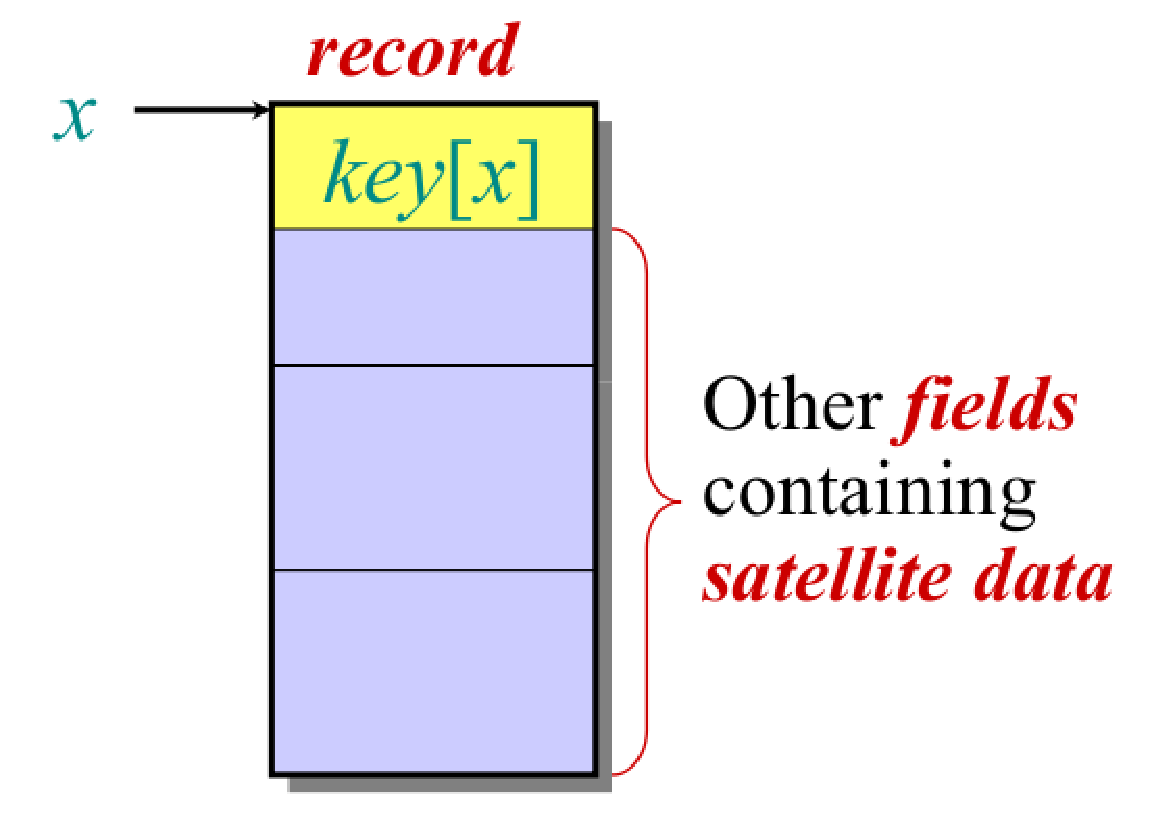
\includegraphics[width=3in]{lecture7/record.eps}
\end{center}

Операции, необходимые для таблицы символов:
\begin{enumerate}
\item Insert(S, x): $S \gets S \cup \lbrace x \rbrace$
\item Delete(S, x): $S \gets S - \lbrace x \rbrace$
\item Search(S, k): возвращает $x$ если $key[x] = k$ \\
  или $nil$ если нет такого $x$
\end{enumerate}

Множество, которое можно изменять с помощью Insert/Delete называется
\emph{динамическим}.

Как должна быть организована таблица символов для того чтобы оптимально
выполнять все эти основные операции?

\section{Таблица с прямой адресацией}
Самой простой имплементацией такой таблицы символов является \emph{таблица с
  прямой адресацией}.

Предположим, что нам необходимо динамическое множество, каждый элемент которого
имеет ключ из множества $U = \lbrace 0, 1, \ldots, m - 1 \rbrace$, где $m$ не
слишком велико. Кроме того предположим, что все ключи различны, то есть никакие
два элемента не имеют одинакового ключа.

Будем использовать массив $T[0 .. m - 1]$ для представления динамического
множества $S$ так, что:

$$ 
T[k] = \begin{cases} x \text{, если } x \in S \text{ и } key[x] = k \\
  nil \text{, в противном случае}
\end{cases}
$$

В таком случае все операции требуют константного времени $\Theta(1)$

Но есть проблема: диапазон ключей может быть очень большим, например 64-битные
числа формируют $2^64$ различных возможных ключей, около 18 квинтиллионов. А
строки -- ещё больше. Таким образом, придётся выделять очень большой массив, что
неприемлемо или часто даже невозможно. При этом большая часть этого массива
останется пустой, т.к. мы используем очень малое его подмножество, к примеру
подмножество имён людей среди множества всех строк до заданной длины.

\section{Хэширование}

Для решения этой проблемы нужно использовать \emph{хэширование}.

Хэш-функция $h(k)$ отображает пространство возможных ключей $U$ на ячейки
(слоты) хэш-таблицы $T[0 .. m - 1]$:

$$
h \colon U \to \lbrace 0, 1, \ldots, m - 1 \rbrace
$$

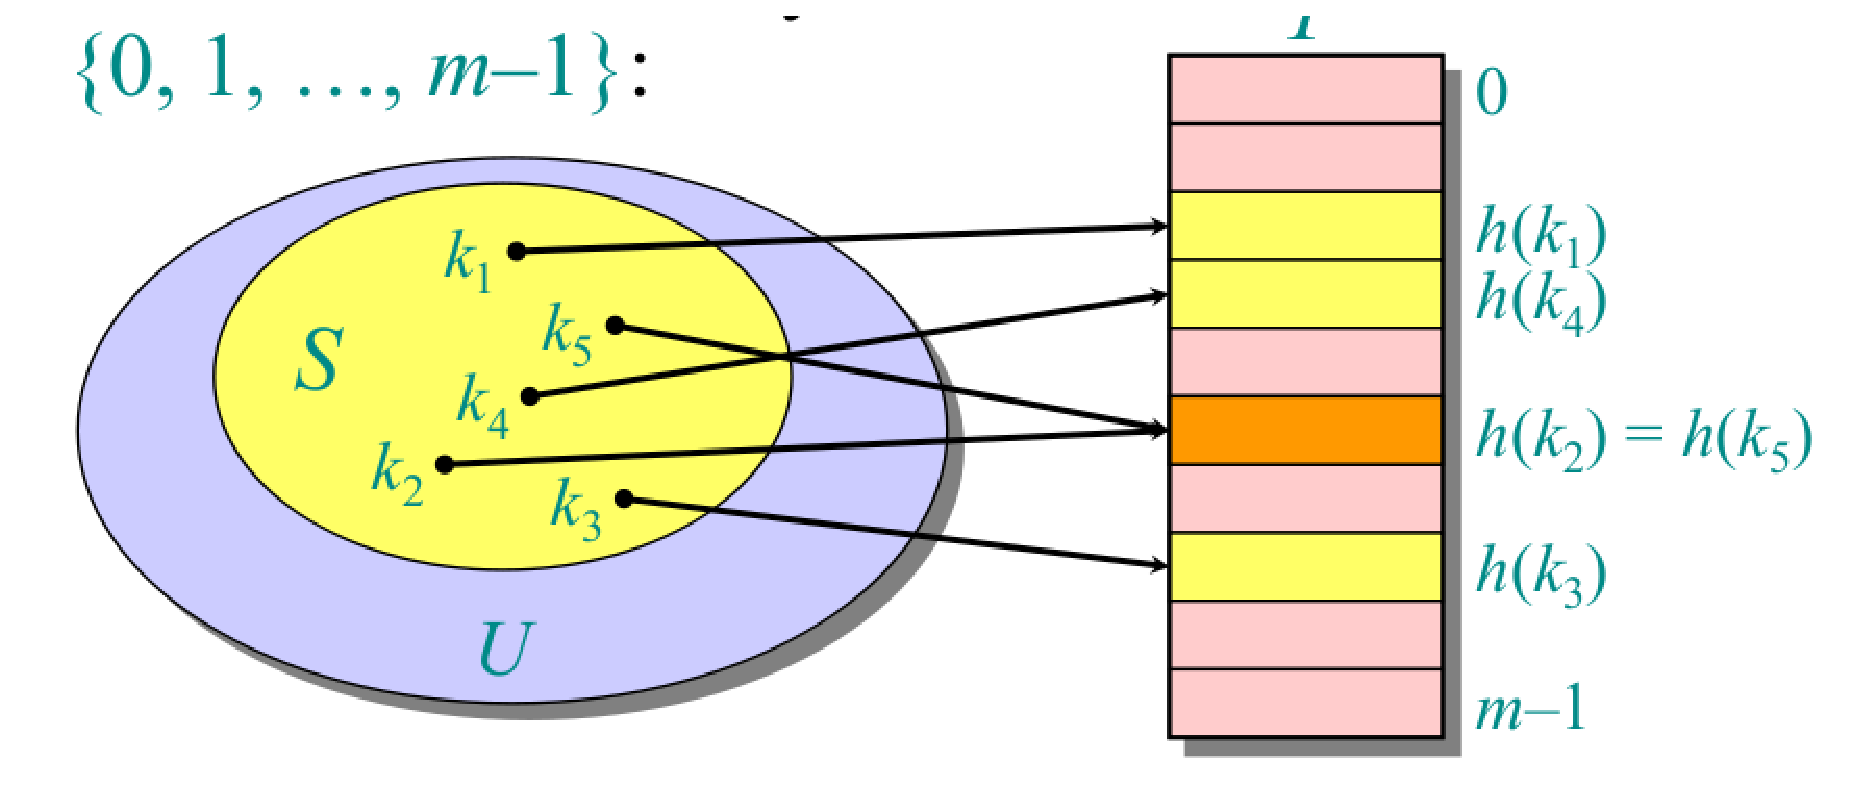
\includegraphics[width=5in]{lecture7/mapping.eps}

Когда два ключа отображаются в одну и ту же ячейку -- мы называем это
\emph{коллизия}.

\section{Разрешение коллизий с помощью цепочек}

Идея состоит в том, чтобы хранить в каждой ячейке не одно значение, а целый
список. И если новый ключ отображается в уже существующую ячейку -- добавлять
его в конец списка.

\begin{center}
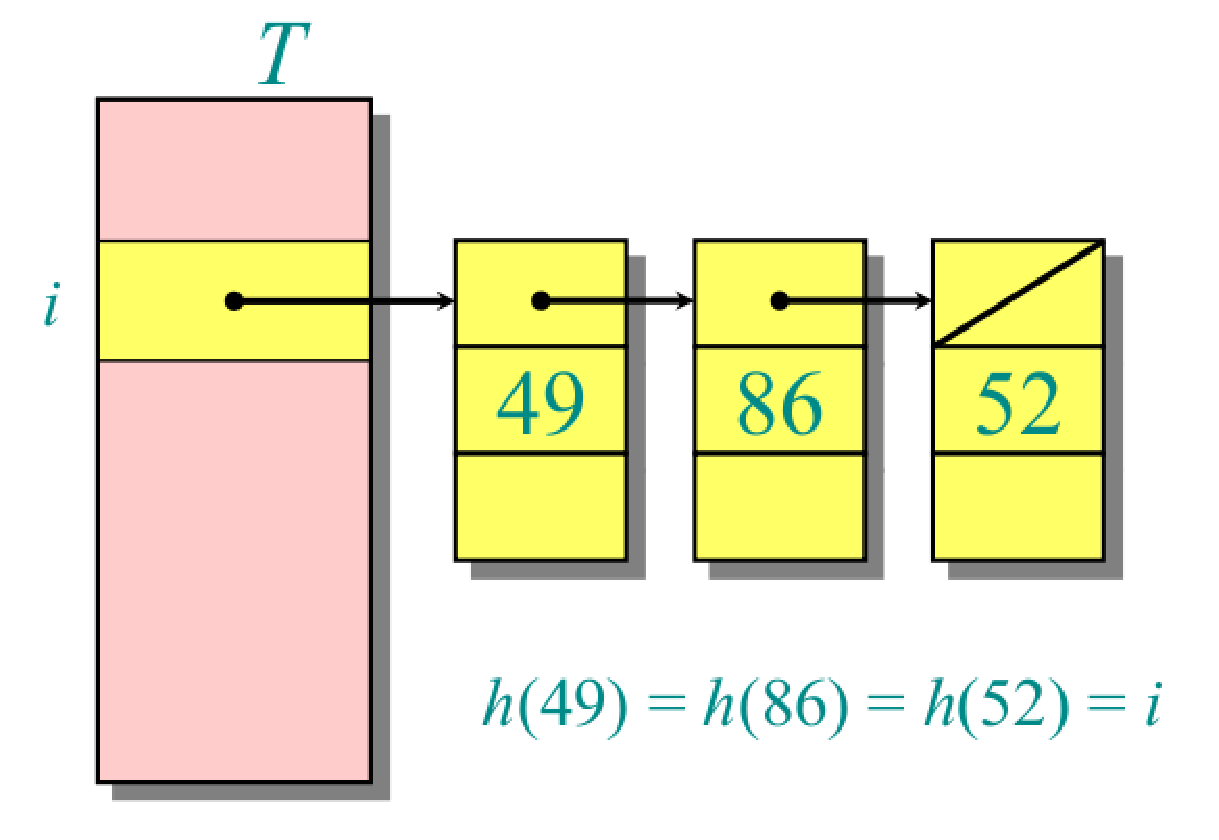
\includegraphics[width=3in]{lecture7/chaining.eps}
\end{center}

\subsection{Анализ}

Анализ худшего случая: все ключи хэшируются в одну и ту же ячейку, мы получаем
вырожденную хэш-таблицу, которая представляет собой просто список. Поиск в
таком списке занимает время $\mathcal{O}(n)$, если $|S| = n$

Анализ среднего случая: когда мы делаем анализ среднего случая, нам всегда нужно
какое-то предположение относительно входных данных, поведения системы в целом.
Здесь нам сложно сделать предположение, поскольку мы сейчас даже не знаем, какая
именно хэш-функция будет использоваться. Однако мы предположим, что мы будем
использовать ``идеальную'' хэш-функцию. Она должна равномерно и независимо
распределять ключи по массиву. Это предположение называется \emph{простым
равномерным хэшированием}:

\begin{itemize}
\item каждый ключ $k \in S$ с равной вероятностью может быть хэшированы в любую ячейку,
  независимо от того, куда попали остальные ключи.
\end{itemize}

Тогда вероятность того, что два ключа попадут в одну и ту же ячейку равна $1/m$

Определим \emph{коэффициент загрузки} (load factor) хэш-таблицы $\alpha$, как
отношение количества возможных ключей $n$ к количеству ячеек в таблице $m$:

$$
\alpha = n / m
$$

Можно сказать, что $\alpha$ -- это среднее количество ключей в одной ячейке таблицы.

Тогда ожидаемое время неуспешного поиска будет равно $\Theta(1 + \alpha)$.
Константное время на вычисления значения хэш-функции плюс время на проход списка
до конца, а т.к. средняя длина массива как раз $\alpha$, то результат равен
$\Theta(1) + \Theta(\alpha) = \Theta(1 + \alpha)$

Таким образом время поиска будет линейным, если $\alpha$ будет линейной, то есть
$n / m = \mathcal{O}(1)$ или $n = \mathcal{O}(m)$

Другими словами, если количество ячеек, как минимум, пропорционально количетсву
элементов, хранящихся в ней, то $n = \mathcal{O}(m)$ и, следовательно, $\alpha
= n/m = \mathcal{O}(m)/m = \mathcal{O}(1)$, а значит поиск элемента в
хэш-таблице в среднем требует линейного времени. Поскольку в худшем случае
вставка элемента в таблицу также $\mathcal{O}(1)$ и удаление в случае
использование двусвязных список так требует $\mathcal{O}(1)$ времени, то можно
сказать, что в среднем все словарные операции в хэш-таблице выполняются за
$\mathcal{O}(1)$

Оказывается, что успешный поиск выполняется за такое же время (доказательство
см. в книге).

\section{Выбор хэш-функции}

Какую бы хэш-функцию мы не выбрали, все равно найдётся последовательность
ключей, которая будет хэшироваться в одну и ту же ячейку. Позже мы рассмотрим
как это можно обойти. Однако на практике часто бывают применимы довольно простые
хэш-функции.

Определим свойства, которые важны для хорошей хэш-функции:

\begin{itemize}
\item должна распределять ключи равномерно по ячейкам
\item закономерности в распределении ключей не должны влиять на равномерность \\
  пример закономерности: все ключи -- чётные числа (например адреса в памяти в
  словах)
\end{itemize}

\subsection{Метод деления}

Популярный простой метод.

$$
h(k) = k \bmod m
$$

Рекомендации:
\begin{itemize}
\item не стоит выбирать $m$ с маленьким простым делителем $d$. \\

  Пример: $d = 2$ и все ключи -- чётные. Тогда получится, что все нечётные
  ячейки таблицы останутся пустыми. \\

  Пример: $d = 2^r$, тогда хэши вообще не зависят от старших бит ключа. Т.к.
  mod по степени двойки $2^r$ -- это по сути получение $r$ младших бит ключа с
  отбрасыванием старших бит.

\item стоит взять $m$ простым числом, не слишком близким к степеням двойки или
  десятки.
\end{itemize}

Есть методы лучше чем этот, т.к. деление -- не самая быстрая операция, умножение
и сложение работают быстрее. Но часто люди используют этот метод, т.к. он очень
простой и его можно прямо ``заинлайнить'' в свой код.

\subsection{Метод умножения}

Пусть $m = 2^r$ и компьютер используется $w$-битовые слова.

Тогда
$$
h(k) = (A \cdot k \bmod 2^w) rsh (w - r)
$$

где $A$ -- нечётное и $2^{w-1} < A < 2^w$

\begin{itemize}
\item не стоит выбирать $А$ слишком близко к $2^{w-1}$ или $2^w$
\item умножение на $2^w$ быстро выполняется
\item оператор $rsh$ тоже быстро выполняется
\end{itemize}

Пример ($m = 2^3 = 8, w = 7$):

\begin{center}
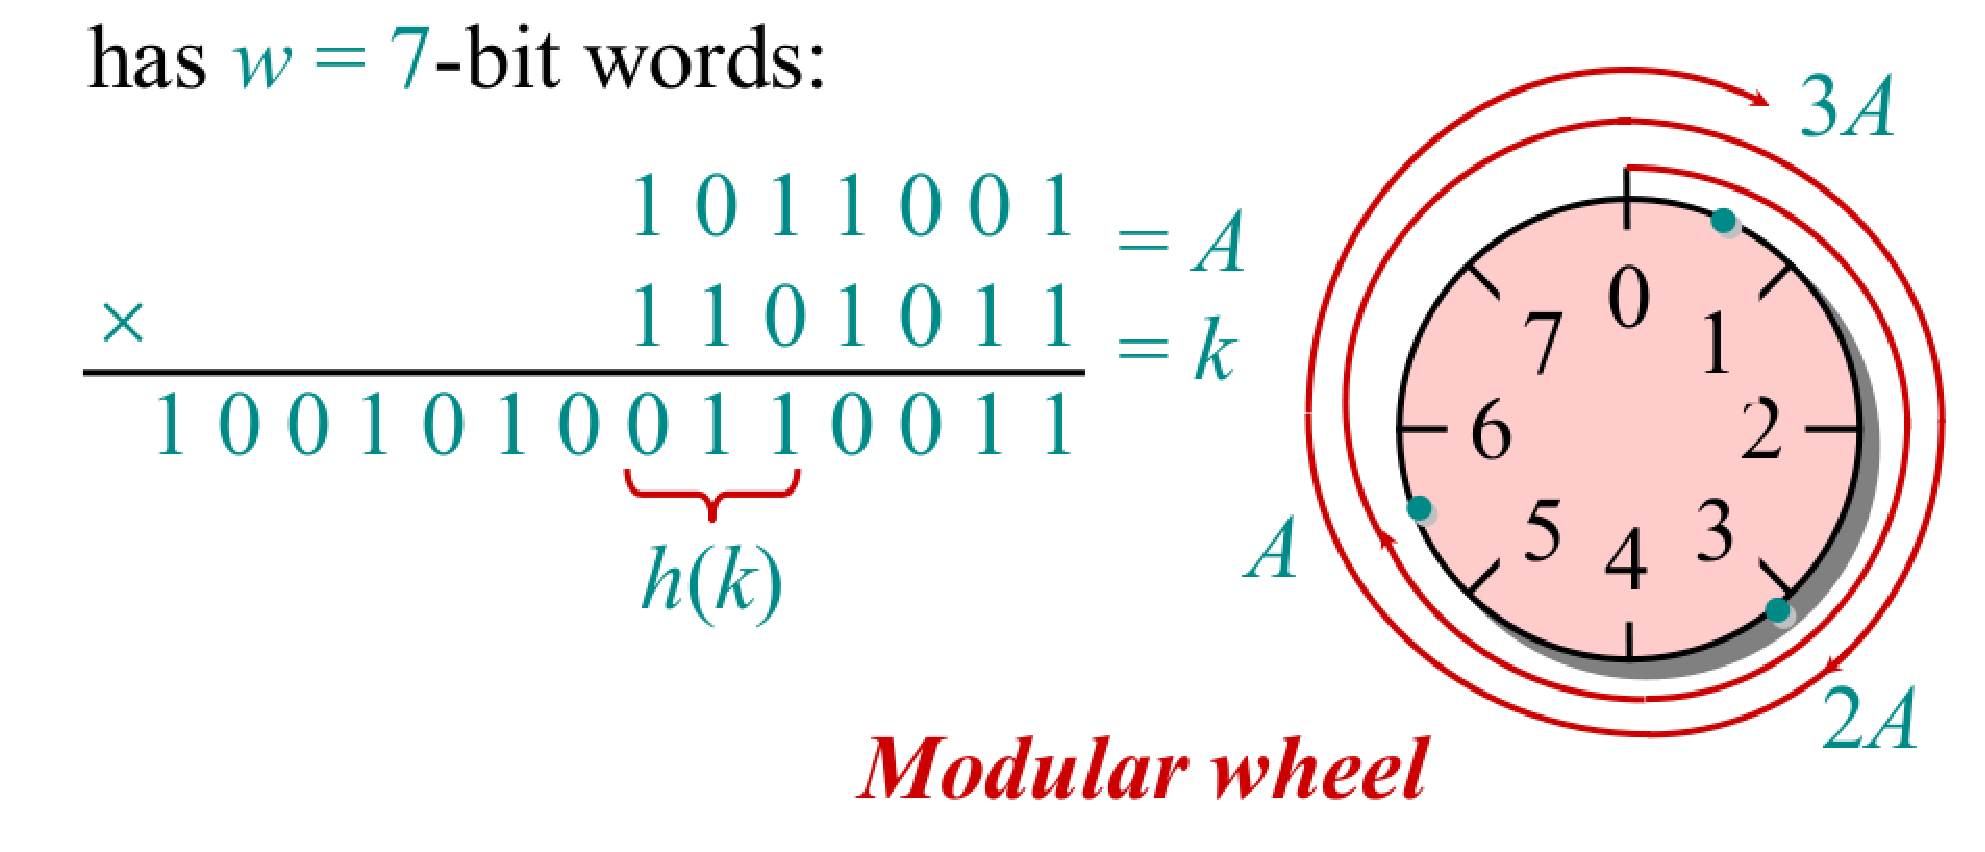
\includegraphics[width=5in]{lecture7/wheel.eps}
\end{center}

Колесо остатков -- равномерно распределяет ключи, почти случайно. При хороших
значениях $A$ получаются отличные результаты.

\section{Разрешение коллизий с помощью открытой адресации}

Не требуется дополнительная память для хранения списков.

Идея: испытываем последовательно ячейки, применяя хэш-функции: если первая
ячейка занята, применяем вторую хэш-функцию и проверяем вторую ячейку -- если
снова занята, то третью и т.д. Набор хэш-функций должен давать перестановку
ячеек, чтобы не нужно было по нескольку раз проверять одно и то же. Рано или
поздно должна найтись пустая ячейка, либо в противном случае -- таблица
полностью заполнена.

Теперь у нас не одна хэш-функция, а последовательность их. Можно сказать, что
теперь хэш-функция принимает не один аргумент, а два: сам ключ и номер попытки,
т.е.:

$$
h \colon U \times \lbrace 0, 1, \ldots, m - 1 \rbrace \to \lbrace 0, 1,
\ldots, m - 1 \rbrace
$$

Соответственно когда мы ищем элементы -- проходим по той же последовательности
ячеек и хэш-функций до тех пор пока не найдём нужный элемент или пустую ячейку.

При этом существует проблема с удалением -- оно возможно, но сложно.

Также стоит учитывать, что таблица может запониться, то есть $n <= m$

Пример:

\begin{center}
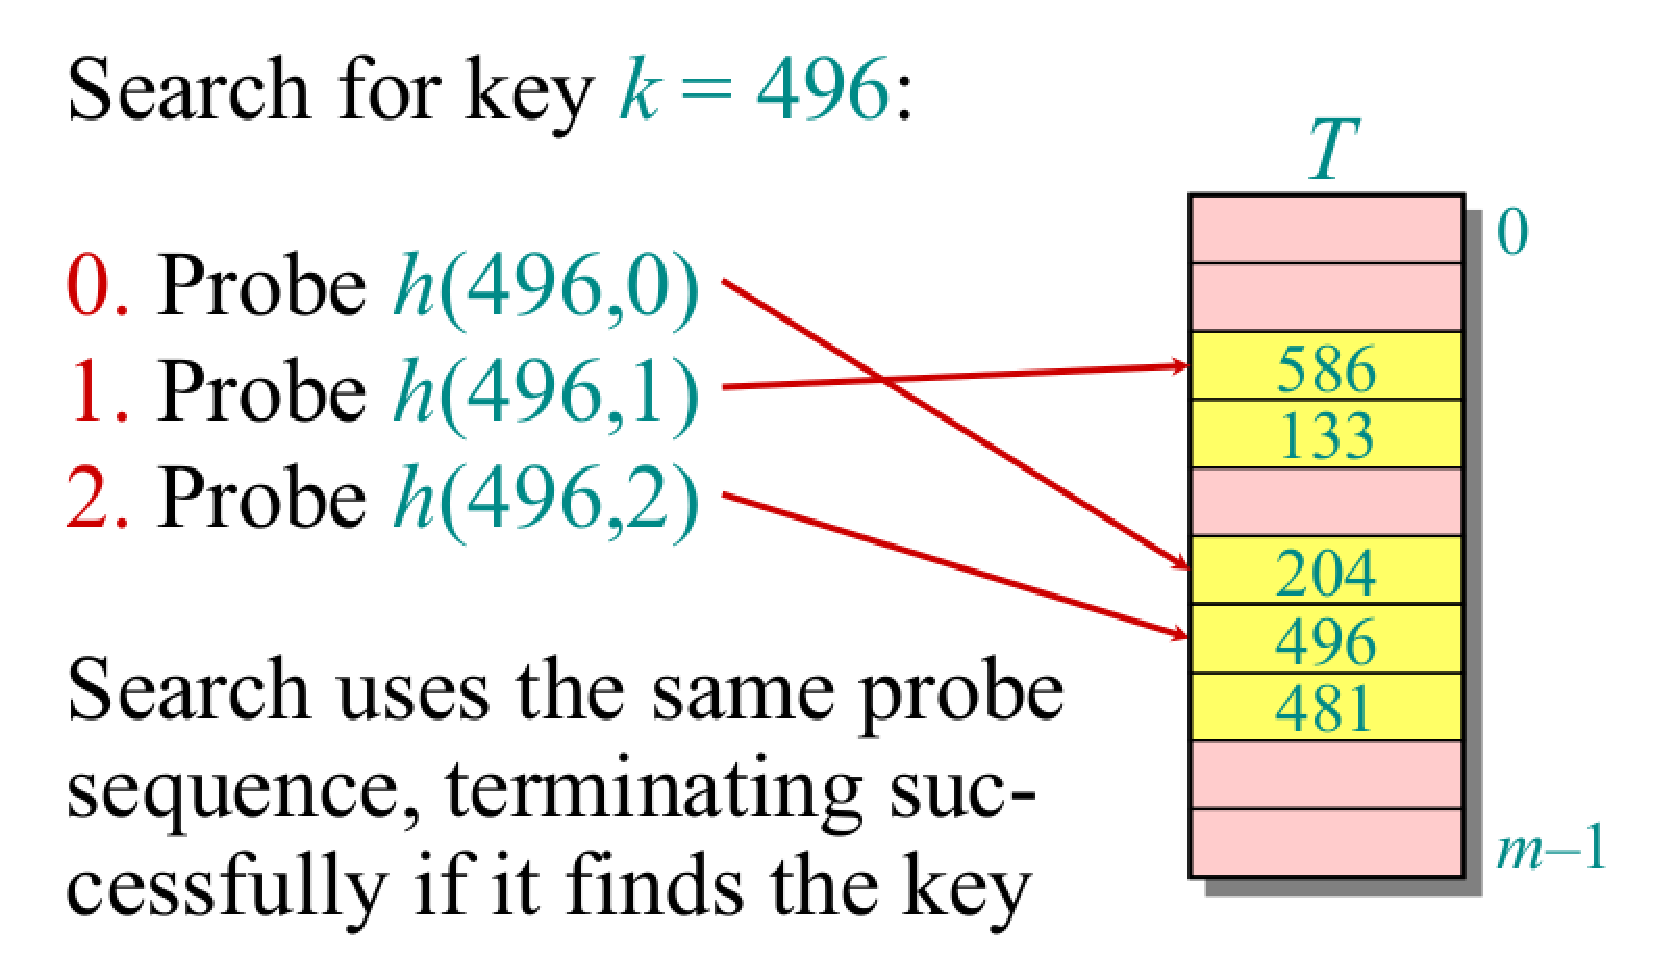
\includegraphics[width=5in]{lecture7/open-addressing.eps}
\end{center}

\section{Стратегии исследования}

\subsection{Линейная стратегия}

$$
h(k, i) = (h'(k) + i) \bmod m
$$

где $h'(k)$ -- обычная хэш-функция.

Данная стратегия легко реализуется, однако подвержено проблеме первчиной
кластеризации, связанной с созданием длинной последовательности занятых ячеек,
что увеличивает среднее время поиска. Кластеры возникают в связи с тем, что
вероятность заполнения ячейки которой предшествуют $i$ заполненных ячеек, равна
$(i+1)/m$. Таким образом, длинные серии имеют тенденцию к ещё большему
удлинению, что и приводит к увеличению среднего времени поиска.

\subsection{Двойное хэширование}

Пусть $h_1(k)$ и $h_2(k)$ -- обычные хэш-функции, тогда

$$
h(k, i) = (h_1(k) + i \cdot h_2(k)) \bmod m
$$

Этот метод даёт отличные результаты, но $h_2(k)$ должен быть взаимно простым с
$m$. Этого можно добиться, используя в качестве $m$ степени двойки и сделав так,
чтобы $h_2(k)$ выдавала только нечётные числа.

\subsection{Анализ}

Для анализа хэширования с открытой адресацией нам понадобится более сильное
предположение: будем считать что используется \emph{равномерное хэширование}, то есть
для каждого ключа равновероятноы все $m!$ возможные последовательности
исследования. То есть последовательность исследований $\langle h(k,0), h(k,1),
\ldots, h(k,m-1) \rangle$, используемая для вставки ключа $k$ с равной
вероятностью является одной из перестановок $\langle 0,1,\ldots,m-1 \rangle$

Используя это предположение, мы докажем теорему.

Теорема: ожидаемое число исследований не превышает $1/(1-\alpha)$, где $\alpha$ --
коэффициент загрузки $ = n/m < 1 $.

Доказательство:

\begin{enumerate}
\item Как минимум требуется хотя бы одно исследование
\item вероятность того что первая ячейка будет занята равна $n/m$
\item вероятность того что вторая будет занята равна $(n-1)/(m-1)$ и т.д.
\item учитываем что $(n - i)/(m - i) < n/m = \alpha $
\end{enumerate}

Таким образом ожидаемое количество исследований равно:

$$
1 + \frac{n}{m} \cdot (1 + \frac{n-1}{m-1} \cdot (1 + \frac{n-2}{m-2} \cdot ( \cdots (1 +
\frac{1}{n-m+1}) \cdots)))
$$

$$
\leq 1 + \alpha \cdot (1 + \alpha \cdot (1 + \alpha(\cdots (1
+ \alpha) \cdots ))) \leq 1 + \alpha + \alpha^2 + \alpha^3 = 1/(1-\alpha)
$$

Следствия теоремы:

\begin{itemize}
\item если $\alpha$ -- константа, то доступ к хэш-таблице с открытой адресацией
  производится за линейное время
\item если таблица наполовину заполнена (наполовину пуста), то в среднем
  количество исследований будет равно $1 / (1 - \alpha) = 1 / (1 - 0.5) = 2$
\item если таблица заполнена на 90 процентов, то в среднем
  количество исследований будет равно $1 / (1 - \alpha) = 1 / (1 - 0.9) = 10$
\end{itemize}

\end{document}

